\section{Pregunta N$^{\circ}$12\qquad Carlos Alonso Aznarán Laos}

\begin{frame}
    \begin{enumerate}\setcounter{enumi}{11}
        \item

              Sea
              \begin{math}
                  f\left(t\right)=
                  \dfrac{1}{1+t^{2}}
              \end{math}
              para $t\in\left[-5,5\right]$, utilizando un polinomio
              interpole $f$ en $n$ puntos igualmente espaciados de
              $\left[-5,5\right]$.
              Considere $n=5,8,10$ y compare con $f$ usando una
              gráfica.
    \end{enumerate}

    \begin{solution}
        \begin{figure}[ht!]
            \centering
            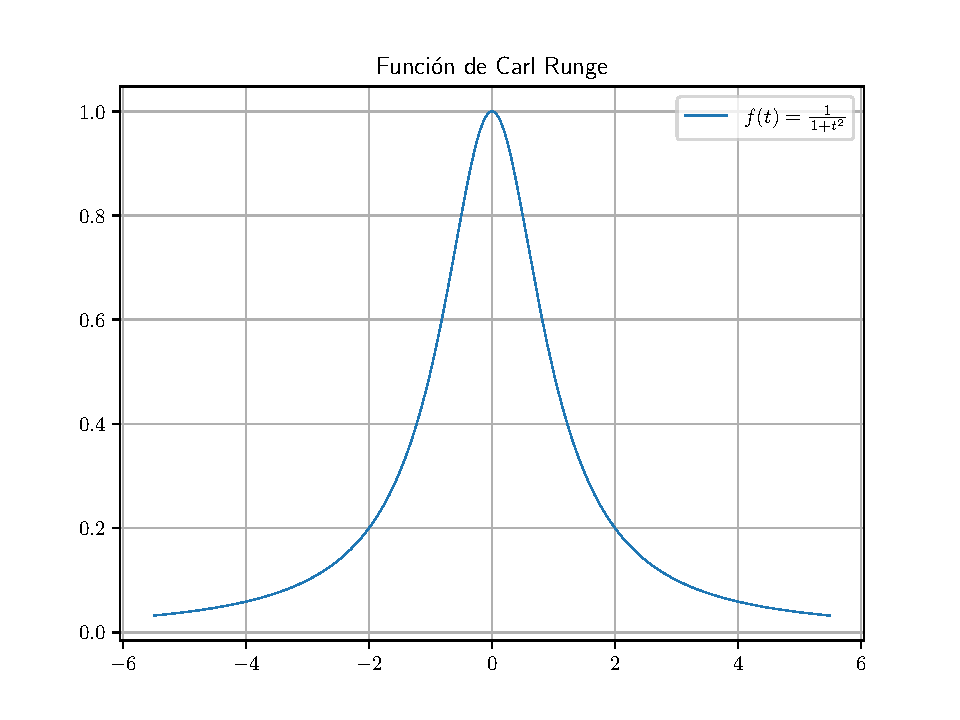
\includegraphics[width=.7\paperwidth]{p12}
        \end{figure}
    \end{solution}
\end{frame}

\begin{frame}
    \begin{solution}
        \begin{figure}[ht!]
            \centering
            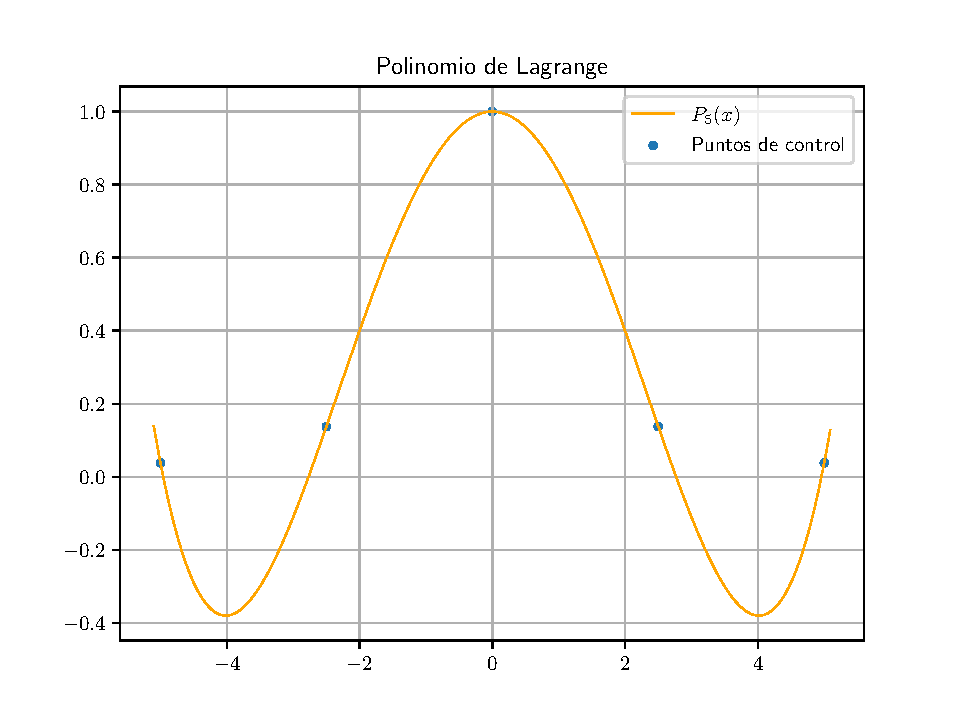
\includegraphics[width=.8\paperwidth]{p12_lagrange5}
        \end{figure}
    \end{solution}
\end{frame}

\begin{frame}
    \begin{solution}
        \begin{figure}[ht!]
            \centering
            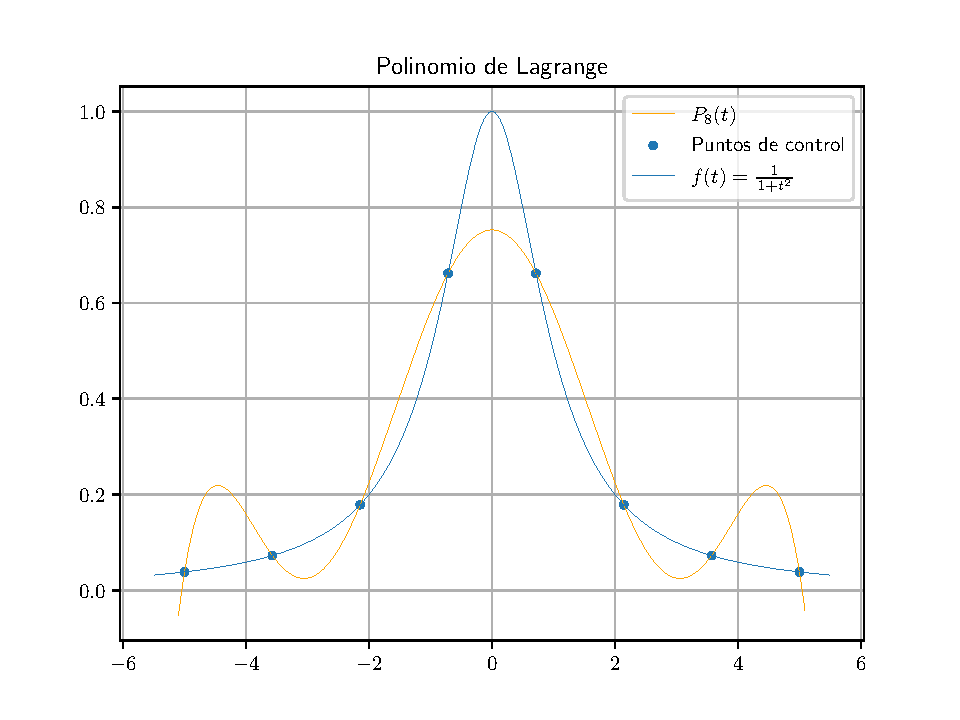
\includegraphics[width=.8\paperwidth]{p12_lagrange8}
        \end{figure}
    \end{solution}
\end{frame}

\begin{frame}
    \begin{solution}
        \begin{figure}[ht!]
            \centering
            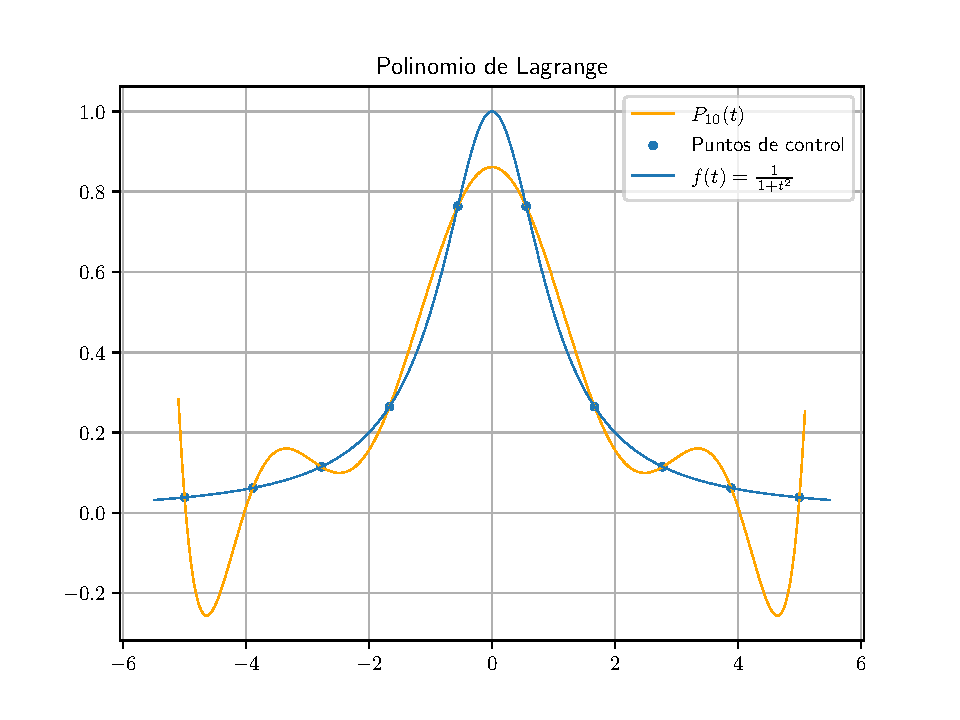
\includegraphics[width=.8\paperwidth]{p12_lagrange10}
        \end{figure}
    \end{solution}
\end{frame}